I am currently in the Ph.D. in Security program at UCCS, with a focus in embedded systems security as it relates to the Experimental Physics \& Industrial Control System (EPICS). I am a firm believer in constant self-improvement through reading and communication while I have a penchant for music as well as poetry. My goal for this class is to become adept at the computer science research process. \par I hope this course will help me understand, in good detail, each stages of the scientific method viz. observation, problem formulation, hypothesis, prediction, testing the prediction, and iteration. I intend to fine tune my skills in each of these processes so that I will be able to make sound observations, ask better research question, design experiments better, foresee impediments ahead of time, and so on and so forth. I also hope to tap into the spangled research dexterity of the instructor, Dr. Boult and to augment my knowledge of presentation.


\begin{figure} [h]
    \captionsetup{justification=centering}
    \centering
    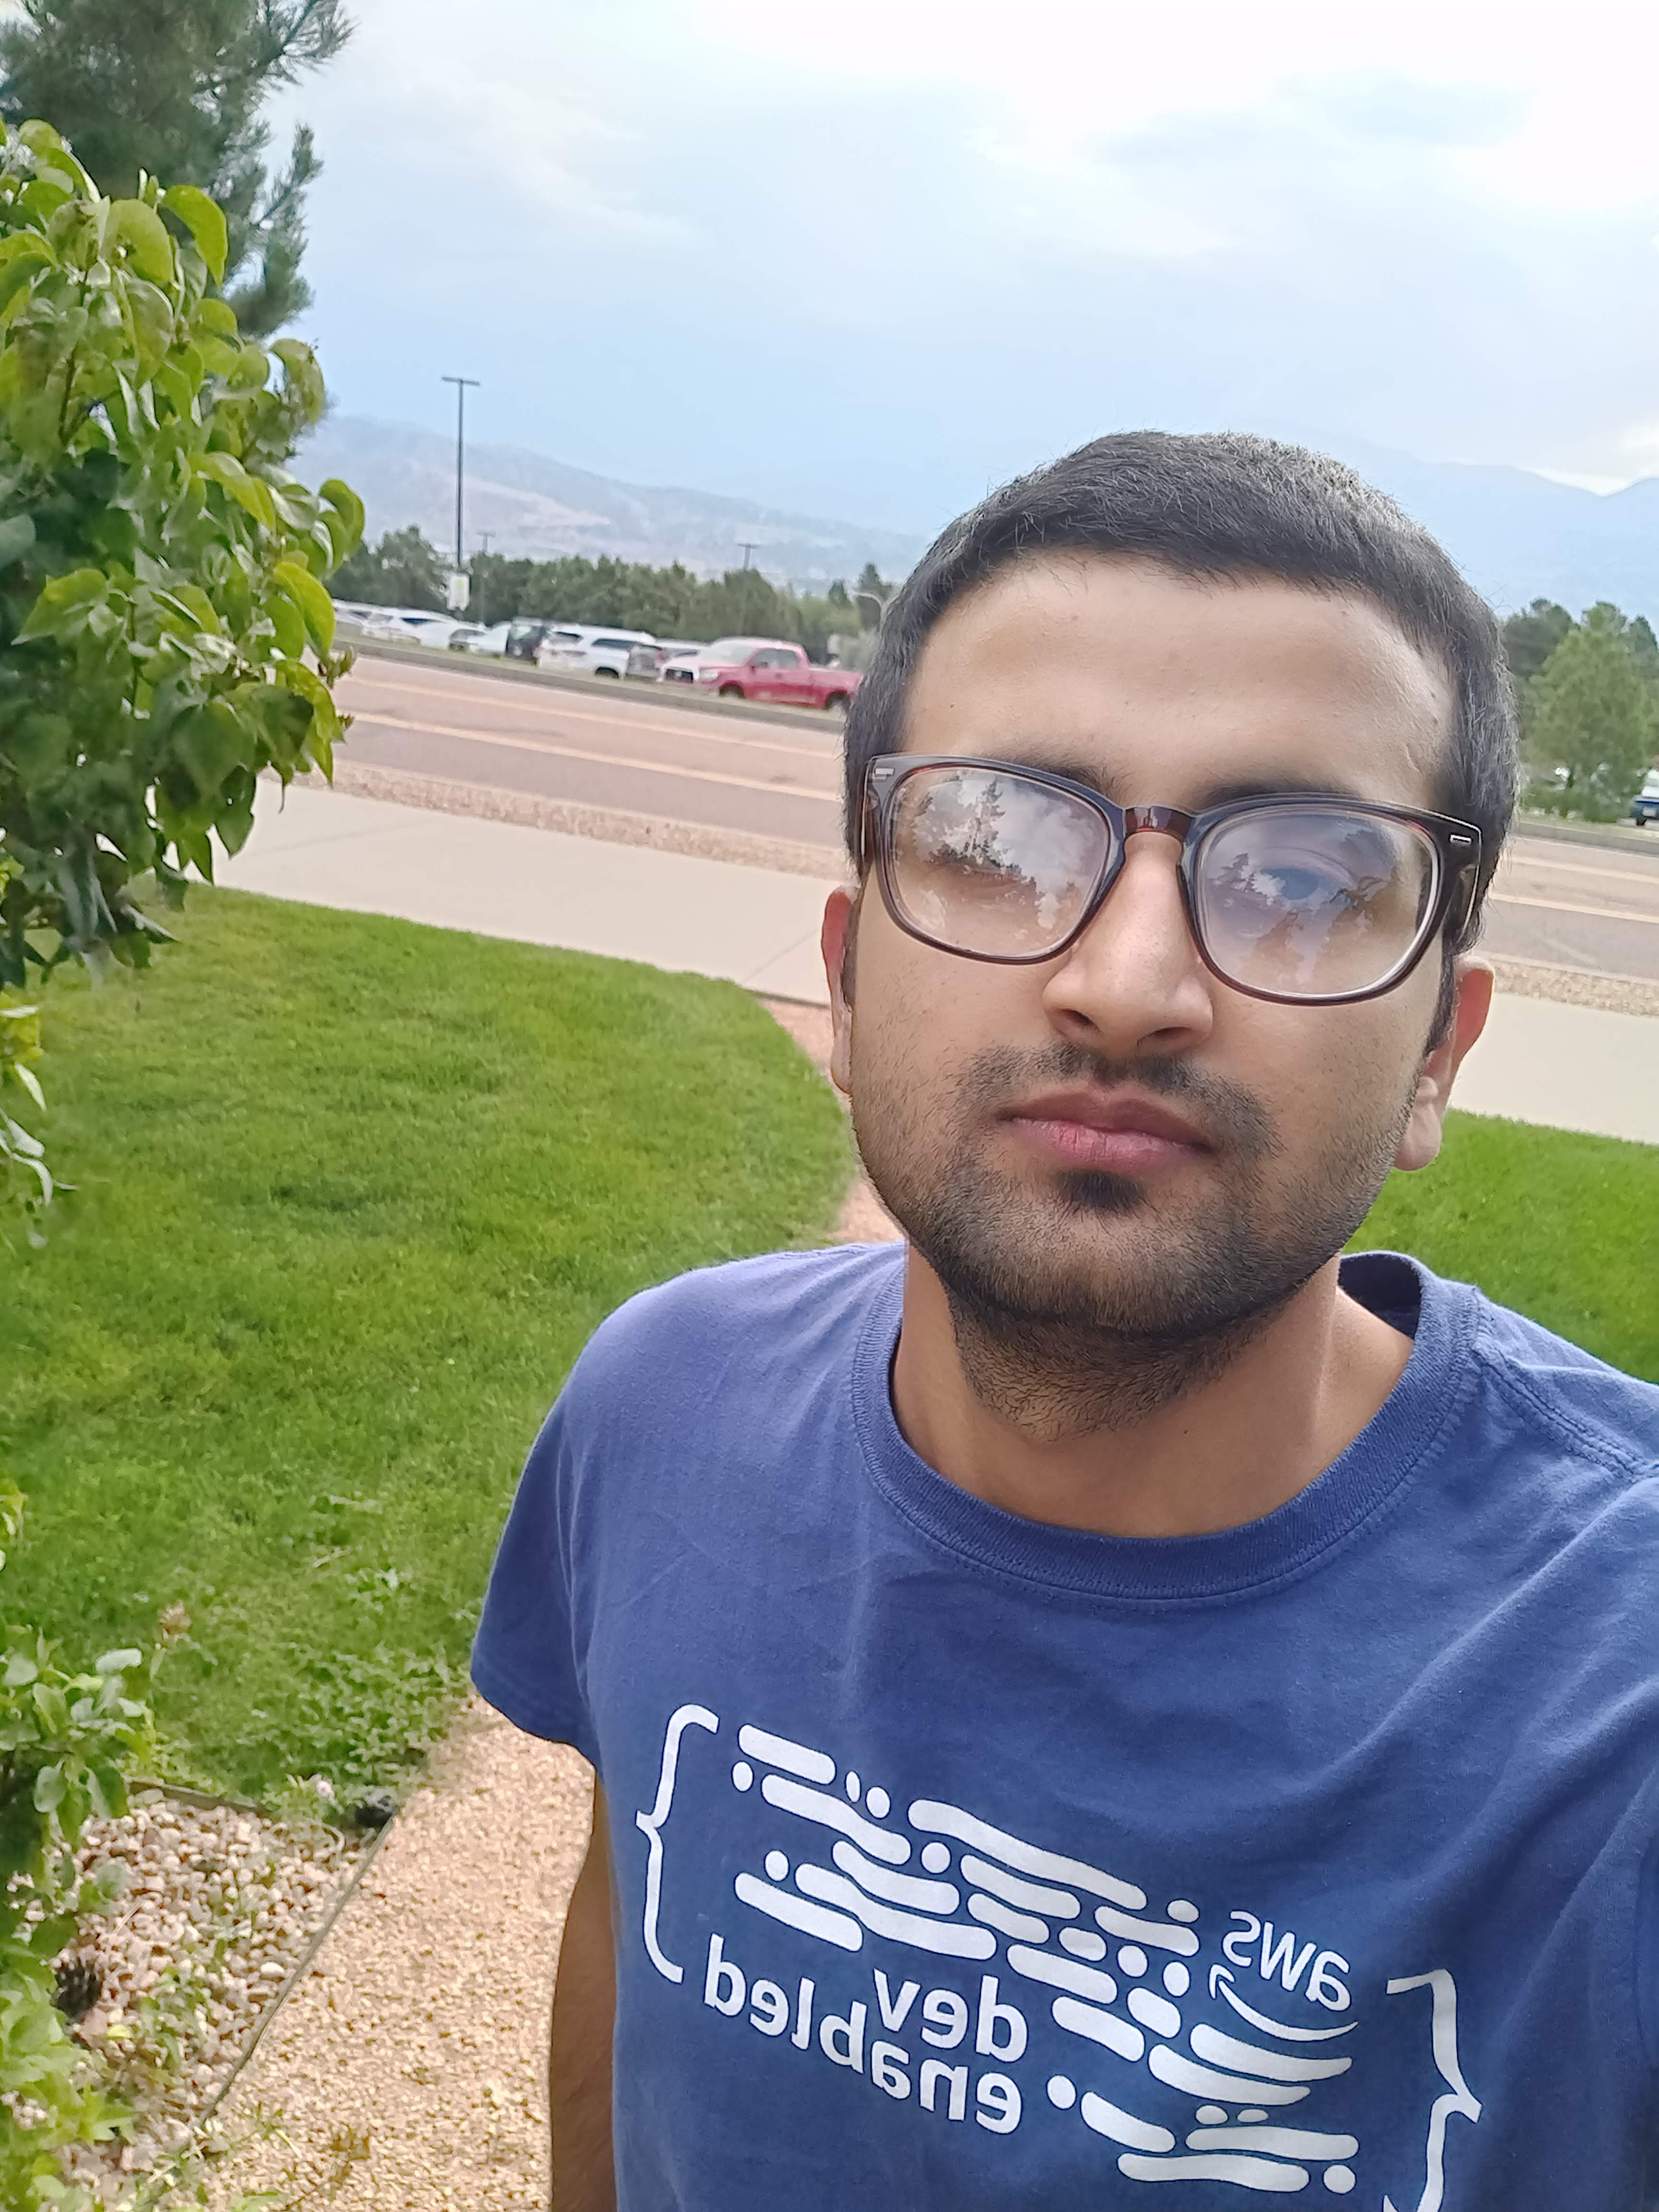
\includegraphics [width= 0.25\textwidth] {Dangal-UCCS}
    \caption{Prajjwal Dangal}
    \label{fig:my_label}
\end{figure}

%\input{Journal 2}

\subsection{Question \& answers for Prajjwal Dangal}

\end{document}
%\endinput
    
    
